\documentclass{article}
  
\usepackage{amsthm}
\theoremstyle{plain} 
   \newtheorem{theorem}{Theorem}[section]
   \newtheorem{corollary}[theorem]{Corollary}
   \newtheorem{lemma}[theorem]{Lemma}
   \newtheorem{proposition}[theorem]{Proposition}
\theoremstyle{definition}
   \newtheorem{definition}[theorem]{Definition}
   \newtheorem{example}[theorem]{Example}
\theoremstyle{remark}    
  \newtheorem{remark}[theorem]{Remark}

\usepackage{amsfonts}
\usepackage{amsmath}
\usepackage{amssymb}
\usepackage{fullpage}
\usepackage{parskip}
\usepackage{graphicx}

\usepackage{xcolor}
\definecolor{dkgreen}{rgb}{0,0.6,0}
\definecolor{gray}{rgb}{0.5,0.5,0.5}
\definecolor{mauve}{rgb}{0.58,0,0.82}
% for the use with lstlean
\definecolor{keywordcolor}{rgb}{0.7, 0.1, 0.1}   % red
\definecolor{tacticcolor}{rgb}{0.0, 0.1, 0.6}    % blue
\definecolor{commentcolor}{rgb}{0.4, 0.4, 0.4}   % grey
\definecolor{symbolcolor}{rgb}{0.0, 0.1, 0.6}    % blue
\definecolor{sortcolor}{rgb}{0.1, 0.5, 0.1}      % green
\definecolor{attributecolor}{rgb}{0.7, 0.1, 0.1} % red

\usepackage{hyperref}
  \hypersetup{
    colorlinks = true,
    urlcolor = blue,       % color of external links using \href
    linkcolor= blue,       % color of internal links 
    citecolor= blue,       % color of links to bibliography
    filecolor= blue,        % color of file links
    }

\usepackage{listings} 
\lstdefinelanguage{haskell}[]{}{
  morekeywords={let,in,if,then,else,case,of,where,module,import,deriving,data,type,newtype,class,instance,null,return,do,pure,guard},
  morestring=[b]",
  morecomment=[l]--,
  morecomment=[n]{/*}{*/},
  basicstyle=\ttfamily,
  keywordstyle=\color{blue}\bfseries,
  stringstyle=\color{red},
  commentstyle=\color{dkgreen},
  identifierstyle=\color{black},
  frame=tb,
  aboveskip=3mm,
  belowskip=3mm,
  columns=flexible,
  basicstyle={\small\ttfamily},
  numbers=none,
  numberstyle=\tiny\color{gray},
  keywordstyle=\color{blue},
  commentstyle=\color{dkgreen},
  stringstyle=\color{mauve},
  breaklines=true,
  breakatwhitespace=true,
  tabsize=3,
}
\lstdefinelanguage{python}{
    commentstyle=\color{dkgreen},
    stringstyle=\color{mauve},
    keywordstyle=\color{blue},
    basicstyle={\small\ttfamily},
    breaklines=true,
    breakatwhitespace=true,
    frame=tb,
    numbers=none,
    tabsize=4,
    morekeywords={import,from,class,def,for,while,if,is,in,elif,else,try,except,finally,print,exec,True,False,None,return,yield,break,continue,pass,raise,with,as,lambda,assert,del,global,nonlocal,not,or,and,self},
    morestring=[b]",
    morestring=[b]',
    morecomment=[l]\#,
    morecomment=[s]{'''}{'''},
    morecomment=[s]{"""}{"""}
}
\def\lstlanguagefiles{lstlean.tex}

\title{Typesetting in LaTeX}
\author{Alexander Kurz  \\ Chapman University}

\date{\today}

\begin{document}

\maketitle

\begin{abstract}
A very short introduction to typesetting in LaTeX for the courses ``Programming Languages'', ``Compiler Construction'' and ``Algorithm Analysis''.
\end{abstract}

\tableofcontents

\section{Introduction}\label{intro}

First you need to \href{https://www.latex-project.org/get/}{download and install} LaTeX.\footnote{Links are typeset in blue, but you can change the layout and color of the links if you locate the  \texttt{hypersetup} command.}
%
For quick experimentation, you can use an online editor such as \href{https://www.overleaf.com/learn}{Overleaf}. But to grade the report I will used the time-stamped tex-files and pdf-files in your git repository.  

LaTeX is a markup language (as is, for example, HTML). The source code is in a \verb+.tex+ file and needs to be compiled for viewing, usually to \verb+.pdf+.

If you want to change the default layout, you need to type commands. For example, \verb+\medskip+ inserts a medium vertical space and \verb+\noindent+ starts a paragraph without indentation.
 
Mathematics is typeset between double dollars, for example $$x+y=y+x.$$

\section{LaTeX Resources}

I start a new subsection, so that you can see how it appears in the table of contents.

\subsection{Subsections}

Sometimes it is good to have subsubsections.

\subsubsection{Itemize and enumerate}

\begin{itemize}
\item This is how you itemize in LaTeX.
\item I think a good way to learn LaTeX is by starting from the template file and build it up step by step. Often stackoverflow will answer your questions. LLMs are great at writing LaTeX code. Here are some further resources:
  \begin{enumerate}
  \item \href{https://www.overleaf.com/learn/latex/Learn_LaTeX_in_30_minutes}{Learn LaTeX in 30 minutes}
  \item \href{https://www.latex-project.org/}{LaTeX – A document preparation system}\end{enumerate}
\end{itemize}

\subsubsection{Typesetting Code}

A typical project will involve code. For the example below I took the LaTeX code from \href{https://stackoverflow.com/a/3175141/4600290}{stackoverflow} and the Haskell code from \href{https://hackmd.io/@alexhkurz/HylLKujCP}{my tutorial}.  

\lstset{language=haskell}
\begin{lstlisting}  
-- run the transition function on a word and a state
run :: (State -> Char -> State) -> State -> [Char] -> State
run delta q [] = q
run delta q (c:cs) = run delta (delta q c) cs 
\end{lstlisting}
%
Short snippets such as \texttt{run :: (State -> Char -> State) -> State -> [Char] -> State} can also be directly fitted into text. For example, \verb@run :: (State -> Char -> State) -> State -> [Char] -> State@ is slightly different in terms of spaces and linebreaking (and can lead to layout that is better avoided), as is
\begin{verbatim}run :: (State -> Char -> State) -> State -> [Char] -> State\end{verbatim}

For more on the topic see \href{https://www.overleaf.com/latex/examples/code-presentations-example-different-ways-shown-in-beamer-metropolis/tsxpnyjbhbds}{Code-Presentations Example}.

Here is a Python example:

\lstset{language=Python}
\begin{lstlisting}
def hello_world():
    print("Hello, World!")  # This is a comment
\end{lstlisting}

Generally speaking,  the methods for displaying code discussed above work well only for short listings of code. For entire programs, it is better to have external links to, for example, Github.


\subsubsection{Typesetting Unicode Characters in Lean Code}

The example below is taken from the \href{https://lean-lang.org/lean4/doc/syntax_highlight_in_latex.html}{Lean Manual}.

\lstset{language=lean}
\begin{lstlisting}
  theorem funext {f₁ f₂ : ∀ (x : α), β x} (h : ∀ x, f₁ x = f₂ x) : f₁ = f₂ := by
    show extfunApp (Quotient.mk f₁) = extfunApp (Quotient.mk f₂)
    apply congrArg
    apply Quotient.sound
    exact h
\end{lstlisting} 


This also works for typesetting Lean code from the Lean Game Server, \href{https://adam.math.hhu.de/#/g/trequetrum/lean4game-logic/world/ImpIntro/level/6}{for example}:

\begin{lstlisting}
  example (C D S: Prop) (h : C ∧ D → S) : C → D → S := by
    exact λ c d ↦ h ⟨c,d⟩ 
\end{lstlisting}

\subsection{Including Images}

It is not possible to include pipes but it is possible to include images, see for example Figure~\ref{pipe}. If you want to allow the image to float to the top of a page insert it in a figure environment. 

\begin{figure}
\begin{center}
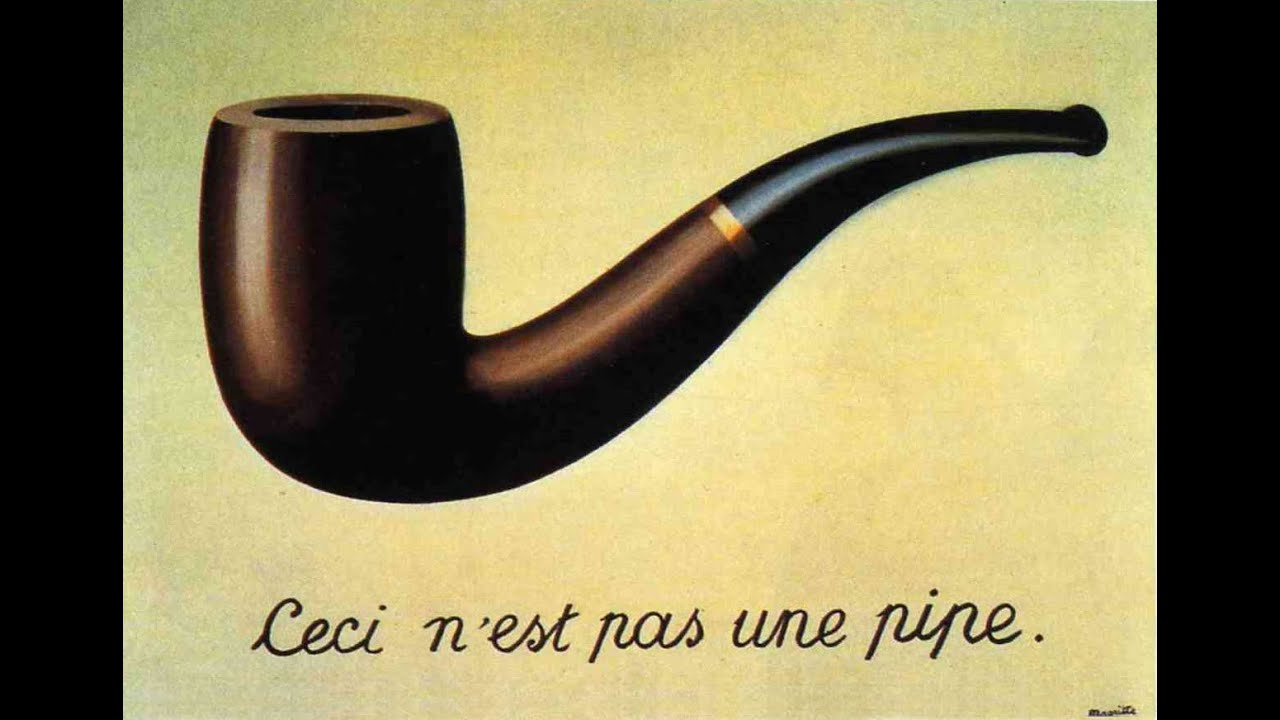
\includegraphics[scale=0.2]{cecinestpasunepipe.jpg}
\end{center}
\caption{Magritte's painting ``This is not a pipe"}\label{pipe}
\end{figure}



\subsubsection{More Mathematics}

We have already seen $x+y=y+x$ as an example of inline maths. We can also typeset mathematics in display mode, for example
$$\frac x y =\frac{xy}{y^2},$$

\noindent
Here is an example of equational reasoning that spans several lines:
\begin{align*}
{\rm fib}(3)
& = {\rm fib}(1) +{\rm fib}(2)  & {\rm fib}(n+2) = {\rm fib}(n)  + {\rm fib}(n+1) \\
& = {\rm fib}(1) +{\rm fib}(0)  + {\rm fib}(1) & {\rm fib}(n+2) = {\rm fib}(n)  + {\rm fib}(n+1) \\
& = 1 + 0  +1 & {\rm fib}(0) = 0,   {\rm fib}(1) = 1\\
& = 2 & {\rm arithmetic}
\end{align*}

\subsubsection{Definitons, Examples, Theorems, Etc}

\begin{definition} 
This is a definition.
\end{definition}

\begin{example}
This is an example.
\end{example}

\begin{proposition}
This is a proposition.
\end{proposition}

\begin{theorem}
This is a theorem.
\end{theorem}

\noindent You can also create your own environment, eg if you want to have Question, Notation, Conjecture, etc.

\section{Plagiarism}

To avoid plagiarism, make sure that in addition to \cite{Alg} you also cite all the external sources you use. Make sure you cite all your references in your text, not only at the end.


\section{Conclusions}\label{conclusions}

In this document, to help you getting started, I gave a first succinct example of typesetting in LaTeX.

\begin{thebibliography}{99}
\bibitem[ALG]{Alg} \href{https://github.com/alexhkurz/algorithm-analysis-2023}{Algorithm Analysis}, Chapman University, 2023.
\end{thebibliography}

\end{document}
